%% Standalone lecture -- build with:  pdflatex -shell-escape biasVariance
%% Shared preamble for standalone lecture files.
%%
%% Every lecture begins with %% Shared preamble for standalone lecture files.
%%
%% Every lecture begins with %% Shared preamble for standalone lecture files.
%%
%% Every lecture begins with \input{preamble} and is compiled on its own:
%%     pdflatex -shell-escape <lecture>
%% There is no master lectures.tex any more -- the list of lectures lives in
%% lectures.yaml and is read by the build scripts.

\documentclass[25pt,landscape,footrule]{foils}
\input{macros_gen}
\backgroundsetup{contents={}}

\usepackage{stmaryrd}
\usepackage{ifthen}
\usepackage{pdf14}

% Every figure lives in this course's lectures/figures (consolidated
% 2026-10-08).  Do not add other courses' folders back: when a name exists in
% several folders LaTeX silently takes the first, which mixed old and new
% frames of the same animation.  A missing figure should be a build error.
\graphicspath{{figures/}{../lectures/figures/}}

\date{}

\newcounter{lessoncnt}
\newcommand{\lesson}[1]{\setcounter{page}{1}%
\section{Mathematics of Machine Learning\\%
\vfill
\textcolor{red}{\textit{#1}}
\vfill}}
 and is compiled on its own:
%%     pdflatex -shell-escape <lecture>
%% There is no master lectures.tex any more -- the list of lectures lives in
%% lectures.yaml and is read by the build scripts.

\documentclass[25pt,landscape,footrule]{foils}
%\usepackage[compat2,pdftex]{geometry}
\usepackage[pdftex]{geometry}
\geometry{headsep=-2.5ex,hscale=0.9,bmargin=2.5cm,tmargin=1cm,textwidth=25cm}
\usepackage[pdftex]{xcolor}
\usepackage{pause}
\usepackage{background}
%\usepackage[color=white]{background}
\usepackage{listings}
\usepackage{graphicx}
\usepackage{epsfig}
\usepackage{epstopdf}
\usepackage{bm}
\usepackage{amssymb}
\usepackage{amsfonts}
\usepackage{marvosym}
\usepackage{cite}
\usepackage{pifont}
\usepackage[english]{babel}
\usepackage{amsmath}
\usepackage{amsfonts}
\usepackage{rotating}
\usepackage{listings}
\usepackage{pp4slide}
%\usepackage{hyperref}
\usepackage{pp4link}
\usepackage{fancyvrb}
\usepackage{multido}
\usepackage{calc}
\usepackage{mleftright}
\mleftright % Redefines \left to \mleft and \right to \mright



\thinmuskip=1mu

\newcommand{\bigstrut}{\rule[-0.5\baselineskip]{0pt}{1.2\baselineskip}}
\renewcommand{\ttdefault}{pcr}

\newcommand{\squeeze}{\setlength{\itemsep}{-2pt}}
%\renewcommand{\familydefault}{cmr}
%\renewcommand{\labelitemii}{\textcolor{green}{$\star$}}
\newcommand{\tick}{{\large \ding{51}}}
\newcommand{\cross}{{\large \ding{55}}}
%\DeclareMathAlphabet{\mat}{OT1}{cmss}{bx}{n}
\DeclareMathAlphabet{\mat}{U}{eur}{b}{n}
\newcommand{\figs}{/home/apb/figures}
\newcommand{\stimes}{{\scriptstyle \times}}
\newcommand{\tr}{\textsf{T}}
\newcommand{\e}[1]{{\rm e}^{#1}}
\newcommand{\E}[1]{{\rm e}^{{\displaystyle #1}}}
\newcommand{\av}[2][]{\mathbb{E}_{#1}\left[ #2 \right]}
\newcommand{\Var}[1]{\mathbb{V}\mathrm{ar}\left( #1 \right)}
\newcommand{\pred}[1]{\left\llbracket { \small #1} \right\rrbracket}
\newcommand{\logg}[1]{\log\left( #1 \right)}
\newcommand{\logtwo}[1]{\log_2\left( #1 \right)}
\newcommand{\bra}[1]{\left( #1 \right)}
\newcommand{\prob}[1]{\mathbb{P}\left( #1 \right)}
\newcommand{\Prob}[1]{\mathbb{P}\left( #1 \right)}
\newcommand{\Step}{\mathop{\mat{\Theta}}}
\newcommand\diag{\mathop{\mathrm{diag}}}
\newcommand{\grad}{\bm{\nabla}}
\newcommand{\gradx}{\bm{\nabla}_{\!\!\scriptscriptstyle \bm{x}}}
\newcommand{\gradw}{\bm{\nabla}_{\!\!\scriptscriptstyle \bm{w}}}
\newcommand{\dd}{\mathrm{d}}
\newcommand{\ii}{\mathrm{i}}
\newcommand{\data}{\mathcal{D}}
\newcommand{\class}{\mathcal{C}}
\newcommand{\hypo}{\mathcal{H}}
\newcommand{\indep}{\perp \!\!\!\! \perp}
\newcommand{\pd}[3][\,]{\frac{\partial^{#1}{#2}}{\partial\,{#3}}}
\newcommand{\normal}[1]{\mathcal{N}\!\left( #1 \right)}
\newcommand{\Dist}[2][Binom]{\mathrm{#1}\left( \strut {#2} \right)}
\newcommand{\brackets}[1]{\!\left( #1 \right)}
\newcommand{\KL}[2]{\mathop{\mathrm{KL}}\left(#1 \big\| #2\right)}
\newcommand{\argmax}{\mathop{\mathrm{argmax}}}
\newcommand{\argmin}{\mathop{\mathrm{argmin}}}
\newcommand{\margin}{\Delta}
\lstnewenvironment{matlab}[1][frame=TB]{\lstset{#1}}{}       
%\renewcommand{\emph}[1]{\textcolor{red}{\textbf{#1}}}
\newcommand{\myskip}[1]{}
\newcommand\mycom[2]{\genfrac{}{}{0pt}{}{#1}{#2}}
\newcommand{\jl}{\lstinline[basicstyle=\ttfamily\color{DarkGreen},%
 keywordstyle=\bfseries\ttfamily\color{DarkGreen}]}
\definecolor{EmphColor}{rgb}{0.0,0.0,1.0}
\renewcommand{\emph}[1]{{\color{EmphColor}\textbf{#1}}}
\newcommand{\len}[1]{\| #1 \|}
\newcommand{\inner}[2]{\left\langle {#1}, {#2}\right\rangle}
\newenvironment{psmallmatrix}{\left(\begin{smallmatrix}}{\end{smallmatrix}\right)}
  

\definecolor{DarkGreen}{rgb}{0,0.5,0}
\definecolor{DarkRed}{rgb}{0,0,0.5}
\definecolor{HighLight}{rgb}{1,0,0}     % yellow
\definecolor{TextColor}{rgb}{0.0,0.1,0.1}     % white
\definecolor{TwoColor}{rgb}{0.0,0.5,0.1}      % used for switching colors

\definecolor{HeadLineColor}{rgb}{1.0,0.0,0.0} % cyan
\definecolor{SpecialColor}{rgb}{0.53,0.81,1.0}
\renewcommand{\normalcolor}{\color{HeadLineColor}}

\pausecolors{TwoColor}{TextColor}{HighLight}
\pausecolors{EmphColor}{TextColor}{EmphColor}
\pausecolors{DarkGreen}{DarkGreen}{DarkRed}
\pausecolors{SpecialColor}{white}{HighLight}

\newenvironment{PauseHighLight}{\color{TwoColor}\pausehighlight}{}
\newcommand{\multipdf}[2][width=\linewidth]{\multiinclude[pause=\pauselevel{:+0}\pause,format=pdf,graphics={#1}]{#2}}

\lstdefinelanguage{pseudo}
 {keywords={all,and,begin,break,continue,do,else,elseif,%
     end,endif,endfor,endwhile,%
     exit,false,for,forall,goto,if,%
     or,return,then,true,to,repeat,until,while},%
  comment=[s]{/*}{*/},%
  morecomment=[l]//,%
  morestring=[d]"%
 }[keywords,comments,strings]


\lstloadlanguages{Java,pseudo,Python}
\lstset{
  basicstyle=\footnotesize\ttfamily\color{DarkGreen},
  keywordstyle=\bfseries\footnotesize\ttfamily\color{DarkGreen},
  commentstyle=\footnotesize\it\rmfamily\color{blue},
  language=Java,
  showstringspaces=false
  }


\lstnewenvironment{pseudo}[1][]{\lstset{language=pseudo,mathescape,literate={:=}{{$\gets$}}2 {!}{{$\neg$}}1 {!=}{{\!\!$\neq$\,\,}}2 {<=}{{\!\!$\leq$\,\,}}2 {>=}{{\!\!$\geq$\,\,}}2,escapechar=\#,#1}}{}
\lstnewenvironment{java}[1][]{\lstset{escapechar=\$,#1}}{}
% Python code: the language setting makes # comments use commentstyle.
% Comments stay monospaced: the default italic roman letter-spaces badly
% on listings' fixed columns.
\lstnewenvironment{python}[1][frame=TB]{\lstset{language=Python,
    commentstyle=\footnotesize\ttfamily\color{blue},#1}}{}

\MyLogo{}
%\Restriction{}
%\rightfooter{\hyperlink{overview}{$\square$}}

\newcommand{\keywords}[1]{\vfill{\noindent\it #1}}

\newcounter{outlineitem}
\setcounter{outlineitem}{0}
\newcommand{\outlineitem}[2]{\item%
  \def\targ{\value{emumi}}%
  \ifnum\value{enumi}=\value{outlineitem}%
  \color{HighLight}\textbf{#1}\toptarget{#2}\color{TextColor}%
   \else\toplink{#2}{#1}\fi
}
\color{TwoColor}


%-- Instead of writing \section we want the file structured by \section.
\newcommand{\section}[2][0]{\foilhead[#1cm]{#2}}

%-- Write each page into a \begin{slide} -- \end{slide} environment.
\newenvironment{slide}{}{\pauselevel{=1}}

\MyLogo{\pauselevel{=1}\Acrobatmenu{GoBack}{%
  \color{TextColor}{Adam Pr\"ugel-Bennett}} \hspace{2cm}
  % Clicking on the name steps one slide back.
  \toplink{firstoutline}{\color{red}Mathematics of Machine
    Learning}%
  \hspace{2cm}
  \texttt{//ecs-vlc.github.io/aice3001/}
  %Clicking on the date jumps to the last page, which should be the
  %table of contents.
  \rightfooter{\Acrobatmenu{LastPage}{\qquad%
  \textsf{\color{TextColor}\tiny\thepage}}}% page number
  % Clicking on the page number steps one slide back.
}
\raggedright
\newcommand{\Outline}{}

\newcommand{\pb}{\pausebuild \color{TwoColor}}
\newcommand{\pauseb}{\pauselevel{build, highlight}\pause}
\newcommand{\hl}[1]{\pauselevel{=1, highlight =1 :1, highlight =#1 :#1}\pause}
\newcommand{\hll}{\pauselevel{=1, highlight =1 :1}\pause}
\newcommand{\pauseh}{\pauselevel{highlight}\pause}
\newcommand{\nhl}[1]{\textcolor{TextColor}{#1}}
\newcommand{\mypl}[1]{\pauselevel{=#1 :#1}\pause}
\input supp-pdf.tex
\DeclareGraphicsRule{*}{mps}{*}{}
\usepackage{mpmulti}
%\leftheader{}
\rightheader{} % no more page numbers on top right


\hypersetup{pdftitle={ECS Lectures},pdfsubject={Machine Learning}
pdfauthor={Adam Prugel-Bennett},pdfkeywords={machine learning},
pdfpagemode={FullScreen},
bookmarksopen=false,
hypertexnames=false,pdfstartview={FitV},colorlinks,linkcolor={blue},
citecolor={green},urlcolor={blue}}



\newcommand\bluepage{
\clearpage
\renewcommand\normalcolor{\color{yellow}}
\pagecolor{blue}
\renewcommand\Black{\color{white}}
\color{white}
\hypersetup{colorlinks=true}
}

\newcommand\whitepage{
\clearpage
\renewcommand\normalcolor{\color{black}}
\pagecolor{white}
\renewcommand\Black{\color{black}}
\color{black}
\hypersetup{colorlinks=true}
}

\whitepage
\setlength{\unitlength}{1mm}

\newenvironment{leftImage}[2][0.3]{%
\begin{minipage}{#1\linewidth}
  \includegraphics[width=\linewidth]{#2}
\end{minipage}\hfill
\begin{minipage}{0.92\linewidth - #1\linewidth}}%
{\end{minipage}}

\newenvironment{rightImage}[2][0.3]{%
\newcommand{\foot}{\begin{minipage}{#1\linewidth}\includegraphics[width=0.98\linewidth]{#2}\end{minipage}}%
\begin{minipage}{0.95\linewidth - #1\linewidth}\raggedright }{\end{minipage}\hfill\foot}


%%% Local Variables: 
%%% mode: latex
%%% TeX-master: t
%%% End: 

\backgroundsetup{contents={}}

\usepackage{stmaryrd}
\usepackage{ifthen}
\usepackage{pdf14}

% Every figure lives in this course's lectures/figures (consolidated
% 2026-10-08).  Do not add other courses' folders back: when a name exists in
% several folders LaTeX silently takes the first, which mixed old and new
% frames of the same animation.  A missing figure should be a build error.
\graphicspath{{figures/}{../lectures/figures/}}

\date{}

\newcounter{lessoncnt}
\newcommand{\lesson}[1]{\setcounter{page}{1}%
\section{Mathematics of Machine Learning\\%
\vfill
\textcolor{red}{\textit{#1}}
\vfill}}
 and is compiled on its own:
%%     pdflatex -shell-escape <lecture>
%% There is no master lectures.tex any more -- the list of lectures lives in
%% lectures.yaml and is read by the build scripts.

\documentclass[25pt,landscape,footrule]{foils}
%\usepackage[compat2,pdftex]{geometry}
\usepackage[pdftex]{geometry}
\geometry{headsep=-2.5ex,hscale=0.9,bmargin=2.5cm,tmargin=1cm,textwidth=25cm}
\usepackage[pdftex]{xcolor}
\usepackage{pause}
\usepackage{background}
%\usepackage[color=white]{background}
\usepackage{listings}
\usepackage{graphicx}
\usepackage{epsfig}
\usepackage{epstopdf}
\usepackage{bm}
\usepackage{amssymb}
\usepackage{amsfonts}
\usepackage{marvosym}
\usepackage{cite}
\usepackage{pifont}
\usepackage[english]{babel}
\usepackage{amsmath}
\usepackage{amsfonts}
\usepackage{rotating}
\usepackage{listings}
\usepackage{pp4slide}
%\usepackage{hyperref}
\usepackage{pp4link}
\usepackage{fancyvrb}
\usepackage{multido}
\usepackage{calc}
\usepackage{mleftright}
\mleftright % Redefines \left to \mleft and \right to \mright



\thinmuskip=1mu

\newcommand{\bigstrut}{\rule[-0.5\baselineskip]{0pt}{1.2\baselineskip}}
\renewcommand{\ttdefault}{pcr}

\newcommand{\squeeze}{\setlength{\itemsep}{-2pt}}
%\renewcommand{\familydefault}{cmr}
%\renewcommand{\labelitemii}{\textcolor{green}{$\star$}}
\newcommand{\tick}{{\large \ding{51}}}
\newcommand{\cross}{{\large \ding{55}}}
%\DeclareMathAlphabet{\mat}{OT1}{cmss}{bx}{n}
\DeclareMathAlphabet{\mat}{U}{eur}{b}{n}
\newcommand{\figs}{/home/apb/figures}
\newcommand{\stimes}{{\scriptstyle \times}}
\newcommand{\tr}{\textsf{T}}
\newcommand{\e}[1]{{\rm e}^{#1}}
\newcommand{\E}[1]{{\rm e}^{{\displaystyle #1}}}
\newcommand{\av}[2][]{\mathbb{E}_{#1}\left[ #2 \right]}
\newcommand{\Var}[1]{\mathbb{V}\mathrm{ar}\left( #1 \right)}
\newcommand{\pred}[1]{\left\llbracket { \small #1} \right\rrbracket}
\newcommand{\logg}[1]{\log\left( #1 \right)}
\newcommand{\logtwo}[1]{\log_2\left( #1 \right)}
\newcommand{\bra}[1]{\left( #1 \right)}
\newcommand{\prob}[1]{\mathbb{P}\left( #1 \right)}
\newcommand{\Prob}[1]{\mathbb{P}\left( #1 \right)}
\newcommand{\Step}{\mathop{\mat{\Theta}}}
\newcommand\diag{\mathop{\mathrm{diag}}}
\newcommand{\grad}{\bm{\nabla}}
\newcommand{\gradx}{\bm{\nabla}_{\!\!\scriptscriptstyle \bm{x}}}
\newcommand{\gradw}{\bm{\nabla}_{\!\!\scriptscriptstyle \bm{w}}}
\newcommand{\dd}{\mathrm{d}}
\newcommand{\ii}{\mathrm{i}}
\newcommand{\data}{\mathcal{D}}
\newcommand{\class}{\mathcal{C}}
\newcommand{\hypo}{\mathcal{H}}
\newcommand{\indep}{\perp \!\!\!\! \perp}
\newcommand{\pd}[3][\,]{\frac{\partial^{#1}{#2}}{\partial\,{#3}}}
\newcommand{\normal}[1]{\mathcal{N}\!\left( #1 \right)}
\newcommand{\Dist}[2][Binom]{\mathrm{#1}\left( \strut {#2} \right)}
\newcommand{\brackets}[1]{\!\left( #1 \right)}
\newcommand{\KL}[2]{\mathop{\mathrm{KL}}\left(#1 \big\| #2\right)}
\newcommand{\argmax}{\mathop{\mathrm{argmax}}}
\newcommand{\argmin}{\mathop{\mathrm{argmin}}}
\newcommand{\margin}{\Delta}
\lstnewenvironment{matlab}[1][frame=TB]{\lstset{#1}}{}       
%\renewcommand{\emph}[1]{\textcolor{red}{\textbf{#1}}}
\newcommand{\myskip}[1]{}
\newcommand\mycom[2]{\genfrac{}{}{0pt}{}{#1}{#2}}
\newcommand{\jl}{\lstinline[basicstyle=\ttfamily\color{DarkGreen},%
 keywordstyle=\bfseries\ttfamily\color{DarkGreen}]}
\definecolor{EmphColor}{rgb}{0.0,0.0,1.0}
\renewcommand{\emph}[1]{{\color{EmphColor}\textbf{#1}}}
\newcommand{\len}[1]{\| #1 \|}
\newcommand{\inner}[2]{\left\langle {#1}, {#2}\right\rangle}
\newenvironment{psmallmatrix}{\left(\begin{smallmatrix}}{\end{smallmatrix}\right)}
  

\definecolor{DarkGreen}{rgb}{0,0.5,0}
\definecolor{DarkRed}{rgb}{0,0,0.5}
\definecolor{HighLight}{rgb}{1,0,0}     % yellow
\definecolor{TextColor}{rgb}{0.0,0.1,0.1}     % white
\definecolor{TwoColor}{rgb}{0.0,0.5,0.1}      % used for switching colors

\definecolor{HeadLineColor}{rgb}{1.0,0.0,0.0} % cyan
\definecolor{SpecialColor}{rgb}{0.53,0.81,1.0}
\renewcommand{\normalcolor}{\color{HeadLineColor}}

\pausecolors{TwoColor}{TextColor}{HighLight}
\pausecolors{EmphColor}{TextColor}{EmphColor}
\pausecolors{DarkGreen}{DarkGreen}{DarkRed}
\pausecolors{SpecialColor}{white}{HighLight}

\newenvironment{PauseHighLight}{\color{TwoColor}\pausehighlight}{}
\newcommand{\multipdf}[2][width=\linewidth]{\multiinclude[pause=\pauselevel{:+0}\pause,format=pdf,graphics={#1}]{#2}}

\lstdefinelanguage{pseudo}
 {keywords={all,and,begin,break,continue,do,else,elseif,%
     end,endif,endfor,endwhile,%
     exit,false,for,forall,goto,if,%
     or,return,then,true,to,repeat,until,while},%
  comment=[s]{/*}{*/},%
  morecomment=[l]//,%
  morestring=[d]"%
 }[keywords,comments,strings]


\lstloadlanguages{Java,pseudo,Python}
\lstset{
  basicstyle=\footnotesize\ttfamily\color{DarkGreen},
  keywordstyle=\bfseries\footnotesize\ttfamily\color{DarkGreen},
  commentstyle=\footnotesize\it\rmfamily\color{blue},
  language=Java,
  showstringspaces=false
  }


\lstnewenvironment{pseudo}[1][]{\lstset{language=pseudo,mathescape,literate={:=}{{$\gets$}}2 {!}{{$\neg$}}1 {!=}{{\!\!$\neq$\,\,}}2 {<=}{{\!\!$\leq$\,\,}}2 {>=}{{\!\!$\geq$\,\,}}2,escapechar=\#,#1}}{}
\lstnewenvironment{java}[1][]{\lstset{escapechar=\$,#1}}{}
% Python code: the language setting makes # comments use commentstyle.
% Comments stay monospaced: the default italic roman letter-spaces badly
% on listings' fixed columns.
\lstnewenvironment{python}[1][frame=TB]{\lstset{language=Python,
    commentstyle=\footnotesize\ttfamily\color{blue},#1}}{}

\MyLogo{}
%\Restriction{}
%\rightfooter{\hyperlink{overview}{$\square$}}

\newcommand{\keywords}[1]{\vfill{\noindent\it #1}}

\newcounter{outlineitem}
\setcounter{outlineitem}{0}
\newcommand{\outlineitem}[2]{\item%
  \def\targ{\value{emumi}}%
  \ifnum\value{enumi}=\value{outlineitem}%
  \color{HighLight}\textbf{#1}\toptarget{#2}\color{TextColor}%
   \else\toplink{#2}{#1}\fi
}
\color{TwoColor}


%-- Instead of writing \section we want the file structured by \section.
\newcommand{\section}[2][0]{\foilhead[#1cm]{#2}}

%-- Write each page into a \begin{slide} -- \end{slide} environment.
\newenvironment{slide}{}{\pauselevel{=1}}

\MyLogo{\pauselevel{=1}\Acrobatmenu{GoBack}{%
  \color{TextColor}{Adam Pr\"ugel-Bennett}} \hspace{2cm}
  % Clicking on the name steps one slide back.
  \toplink{firstoutline}{\color{red}Mathematics of Machine
    Learning}%
  \hspace{2cm}
  \texttt{//ecs-vlc.github.io/aice3001/}
  %Clicking on the date jumps to the last page, which should be the
  %table of contents.
  \rightfooter{\Acrobatmenu{LastPage}{\qquad%
  \textsf{\color{TextColor}\tiny\thepage}}}% page number
  % Clicking on the page number steps one slide back.
}
\raggedright
\newcommand{\Outline}{}

\newcommand{\pb}{\pausebuild \color{TwoColor}}
\newcommand{\pauseb}{\pauselevel{build, highlight}\pause}
\newcommand{\hl}[1]{\pauselevel{=1, highlight =1 :1, highlight =#1 :#1}\pause}
\newcommand{\hll}{\pauselevel{=1, highlight =1 :1}\pause}
\newcommand{\pauseh}{\pauselevel{highlight}\pause}
\newcommand{\nhl}[1]{\textcolor{TextColor}{#1}}
\newcommand{\mypl}[1]{\pauselevel{=#1 :#1}\pause}
\input supp-pdf.tex
\DeclareGraphicsRule{*}{mps}{*}{}
\usepackage{mpmulti}
%\leftheader{}
\rightheader{} % no more page numbers on top right


\hypersetup{pdftitle={ECS Lectures},pdfsubject={Machine Learning}
pdfauthor={Adam Prugel-Bennett},pdfkeywords={machine learning},
pdfpagemode={FullScreen},
bookmarksopen=false,
hypertexnames=false,pdfstartview={FitV},colorlinks,linkcolor={blue},
citecolor={green},urlcolor={blue}}



\newcommand\bluepage{
\clearpage
\renewcommand\normalcolor{\color{yellow}}
\pagecolor{blue}
\renewcommand\Black{\color{white}}
\color{white}
\hypersetup{colorlinks=true}
}

\newcommand\whitepage{
\clearpage
\renewcommand\normalcolor{\color{black}}
\pagecolor{white}
\renewcommand\Black{\color{black}}
\color{black}
\hypersetup{colorlinks=true}
}

\whitepage
\setlength{\unitlength}{1mm}

\newenvironment{leftImage}[2][0.3]{%
\begin{minipage}{#1\linewidth}
  \includegraphics[width=\linewidth]{#2}
\end{minipage}\hfill
\begin{minipage}{0.92\linewidth - #1\linewidth}}%
{\end{minipage}}

\newenvironment{rightImage}[2][0.3]{%
\newcommand{\foot}{\begin{minipage}{#1\linewidth}\includegraphics[width=0.98\linewidth]{#2}\end{minipage}}%
\begin{minipage}{0.95\linewidth - #1\linewidth}\raggedright }{\end{minipage}\hfill\foot}


%%% Local Variables: 
%%% mode: latex
%%% TeX-master: t
%%% End: 

\backgroundsetup{contents={}}

\usepackage{stmaryrd}
\usepackage{ifthen}
\usepackage{pdf14}

% Every figure lives in this course's lectures/figures (consolidated
% 2026-10-08).  Do not add other courses' folders back: when a name exists in
% several folders LaTeX silently takes the first, which mixed old and new
% frames of the same animation.  A missing figure should be a build error.
\graphicspath{{figures/}{../lectures/figures/}}

\date{}

\newcounter{lessoncnt}
\newcommand{\lesson}[1]{\setcounter{page}{1}%
\section{Mathematics of Machine Learning\\%
\vfill
\textcolor{red}{\textit{#1}}
\vfill}}


\begin{document}

\lesson{When Machine Learning Works}
\vspace{-1cm}
\begin{center}
\noindent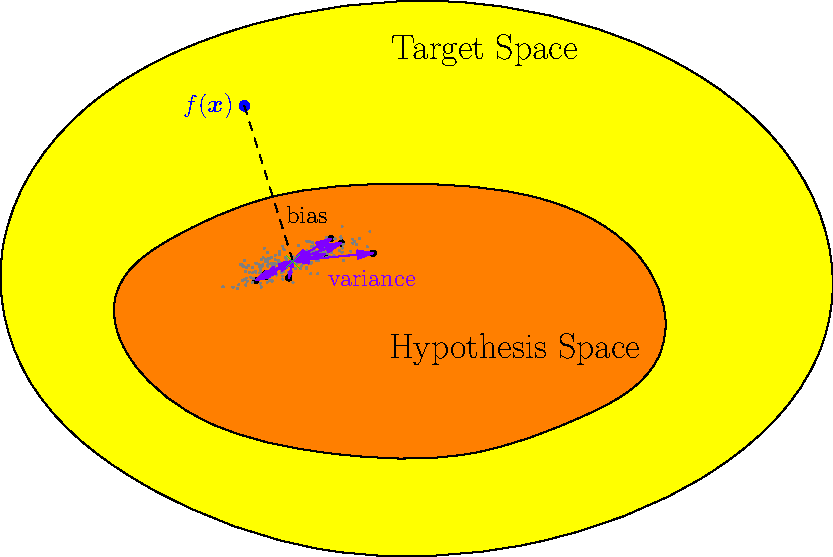
\includegraphics[height=100mm]{approxEstim-21}
\end{center}
\keywords{When ML Works, Bias Variance}
%%%%%%%%%%%%%%%%%%%%%%% Next Slide %%%%%%%%%%%%%%%%%%%%%%%
\renewcommand{\Outline}{%
\begin{slide}
\section[1]{Outline}

\begin{minipage}{12cm}\raggedright
  \begin{enumerate}\squeeze
    \outlineitem{What Makes a Good Learning Machine?}{why}
    \outlineitem{Bias-Variance Dilemma}{dilemma}
    \outlineitem{Shrinkage and Ridge Regression}{examples}
    \outlineitem{Ensembles}{ensembles}
  \end{enumerate}
\end{minipage}\hfill
\begin{minipage}{10cm}
  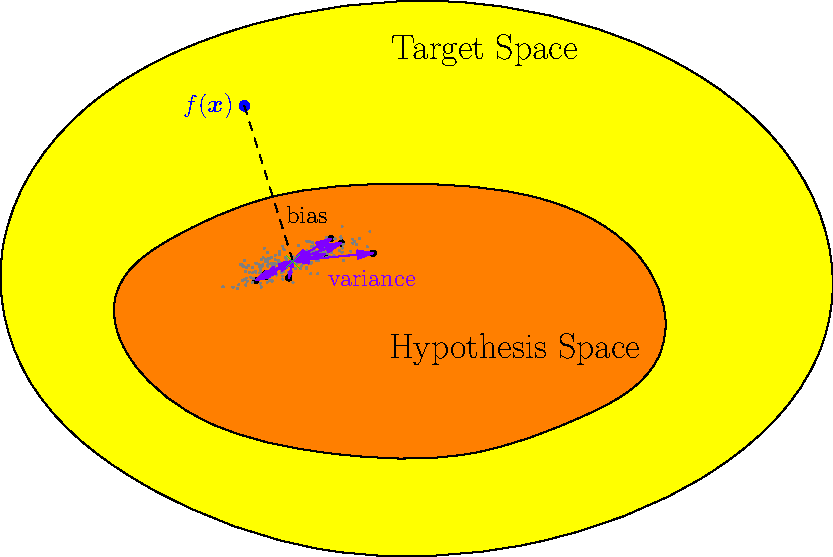
\includegraphics[width=10cm]{approxEstim-21}
\end{minipage}
\end{slide}
\addtocounter{outlineitem}{1}
}

\setcounter{outlineitem}{1}

%%%%%%%%%%%%%%%%%%%%%%% Next Slide %%%%%%%%%%%%%%%%%%%%%%%
\Outline % Why ML works
\toptarget{firstoutline}
%%%%%%%%%%%%%%%%%%%%%%% Next Slide %%%%%%%%%%%%%%%%%%%%%%%


\begin{slide}
\section{What Makes a Good Learning Machine?}

\begin{PauseHighLight}
  \begin{itemize}
  \item We want to understand why some machine learning techniques
    work well and others don't\pause
  \item To understand why they work we need to understand what makes a
    good learning machine\pause
  \item For this we have to get conceptual and think about
    \emph{generalisation} performance\pause
    \begin{quote}\it
      \textbf{generalisation}: how well do we do on unseen data as
      opposed to the training data\pause
    \end{quote}
  \end{itemize}
\end{PauseHighLight}

\end{slide}

%%%%%%%%%%%%%%%%%%%%%%% Next Slide %%%%%%%%%%%%%%%%%%%%%%%

\begin{slide}
\section{What Makes Machine Learning Hard?}

\begin{PauseHighLight}
  \begin{itemize}
  \item Typically we work in high dimensions (i.e. have many
    features)\pause
  \item The problem can be over-constrained (i.e. we have conflicting
    data to deal with)\pause---solve by minimising an error function\pauseb
  \item The problem can be under-constrained (i.e. there are many
    possible solutions that are consistent with the data)\pause---need to
    choose a plausible solution\pauseb
  \item Typically in machine learning the data will be over-constrained
    in some dimensions and under-constrained in others\pause
  \item We can't visualise the data to know what is going
    on\pause
  \end{itemize}
\end{PauseHighLight}

\end{slide}

%%%%%%%%%%%%%%%%%%%%%%% Next Slide %%%%%%%%%%%%%%%%%%%%%%%

\begin{slide}
\section{Least Squares}

\begin{PauseHighLight}
  \begin{itemize}
  \item Suppose we want to learn some output $y$ for a feature vector $\bm{x}$\pause
  \item We construct a learning machine that makes a prediction
    $\hat{f}(\bm{x}|\bm{\theta})$\pause
  \item We typically choose the machine to  minimise a \textit{training loss}
    \begin{align*}
      L_T(\mathcal{D}) = \sum_{(\bm{x},y)\in\mathcal{D}} \left(
      \hat{f}(\bm{x}|\bm{\theta}) - y \right)^2 \pause
      = \sum_{i=1}^m \left(
      \hat{f}(\bm{x}_i|\bm{\theta}) - y_i \right)^2
    \end{align*}
    where $\mathcal{D} = \{(\bm{x}_i, y_i)\}_{i=1}^m$ is a set of
    size $m$, sampled from a probability distribution $\mu(\bm{x},y)$\pauseb
  \item We call this machine $\hat{f}(\bm{x}\vert \bm{\theta}_\mathcal{D})$\pauseb
  \end{itemize}
\end{PauseHighLight}

\end{slide}

%%%%%%%%%%%%%%%%%%%%%%% Next Slide %%%%%%%%%%%%%%%%%%%%%%%

\begin{slide}
\section{Generalisation Error}

\begin{PauseHighLight}
  \begin{itemize}
  \item We want to minimise the \textit{generalisation loss} which in
    this case is
    
    \begin{rightImage}{sampleSpace}
      \begin{align*}
        L_G(\bm{\theta}_{\mathcal{D}}) &= \sum_{(\bm{x},y)\in\mathcal{Z}} \mu(\bm{x},y)\,
        \left(\hat{f}(\bm{x}\vert \bm{\theta}_\mathcal{D}) - y
        \right)^2\pause \\
        \mu(\bm{x}, y) &= p(y|\bm{x})\,p(\bm{x})\pauseb
      \end{align*}
    \end{rightImage}\pause

    (we can estimate this if we have some labelled examples
    $(\bm{x}_i,y_i)$ which we have not trained on)\pauseb
  \item We want to minimise $L_G(\bm{\theta}_{\mathcal{D}})$ but in practice we areb
    minimising $L_T(\mathcal{D})$\pause, \textit{what could possibly go wrong?}\pauseb
  \end{itemize}
\end{PauseHighLight}

\end{slide}

%%%%%%%%%%%%%%%%%%%%%%% Next Slide %%%%%%%%%%%%%%%%%%%%%%%

\begin{slide}
\section[-2]{Too Simple or Too Complex?}

\pb
\hypertarget{regression}{}

\begin{itemize}
\item Fit $\hat{f}(x|\bm{\theta}_\mathcal{D})$ to data\pauseh
  \begin{center}
    \multipdf{curveFitting}\pause
  \end{center}
\end{itemize}

\end{slide}


%%%%%%%%%%%%%%%%%%%%%%% Next Slide %%%%%%%%%%%%%%%%%%%%%%%

\begin{slide}
\section[-1]{Measuring Generalisation Error for Regression}

\begin{PauseHighLight}

\begin{itemize}
\item Consider the regression example.  The root mean squared error
  is
  \begin{center}
    \noindent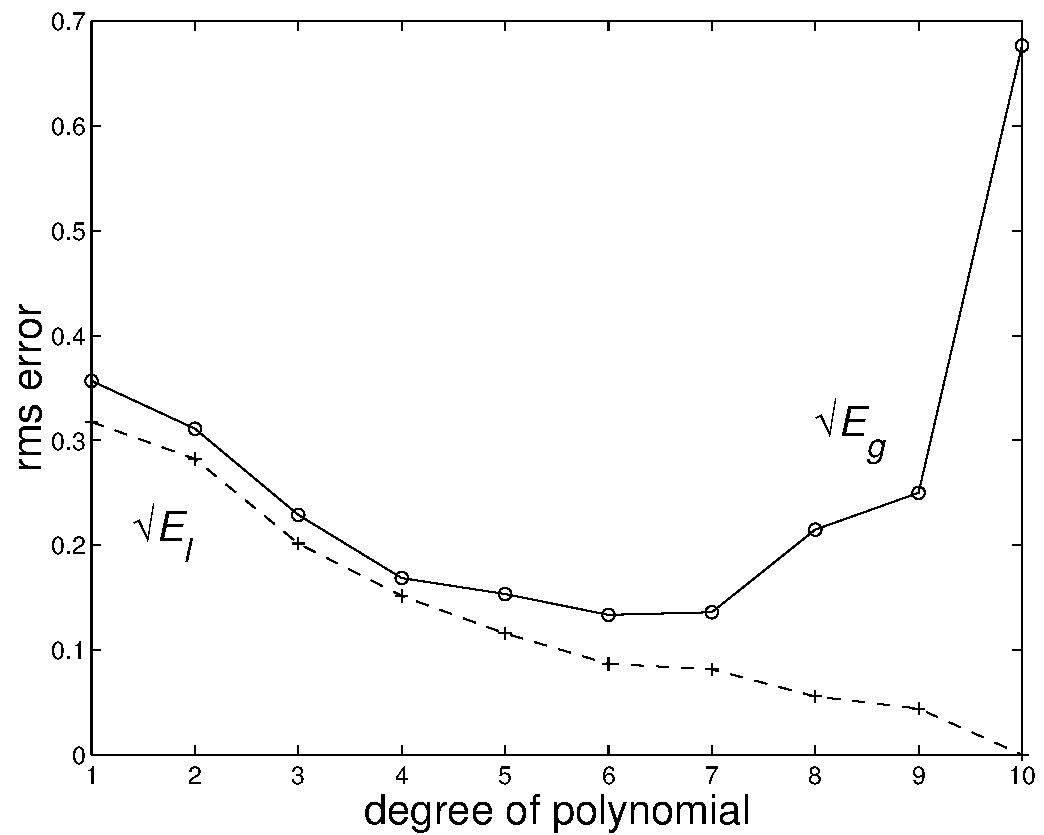
\includegraphics[height=120mm]{rmsErrors}
  \end{center}\pause
\end{itemize}

\end{PauseHighLight}
\end{slide}

%%%%%%%%%%%%%%%%%%%%%%% Next Slide %%%%%%%%%%%%%%%%%%%%%%%
\Outline % Bias-Variance Dilemma
%%%%%%%%%%%%%%%%%%%%%%% Next Slide %%%%%%%%%%%%%%%%%%%%%%%

\begin{slide}
\section{Expected Generalisation Performance}

\begin{PauseHighLight}
  \begin{itemize}
  \item Our generalisation performance will depend on our training set,
    $\mathcal{D}$\pause
  \item To reason about generalisation we can ask what is the
    \textit{expected generalisation loss}, when we average over
    all different data sets of size $m$ drawn independently from
    $\mu(\bm{x},y)$\pause
  \item For each data set, $\mathcal{D}$, we would learn a different
    approximator $\hat{f}(\bm{x}\vert \bm{\theta}_\mathcal{D})$\pause
  \item Note that in practice we only get one data set.  We might be
    lucky and do better than the expected generalisation or we might be
    unlucky and do worse\pause
  \end{itemize}
\end{PauseHighLight}

\end{slide}

%%%%%%%%%%%%%%%%%%%%%%% Next Slide %%%%%%%%%%%%%%%%%%%%%%%

\begin{slide}
\section[-2]{Approximation and Estimation Errors}
\pb\pause\pauselevel{=1}
\begin{center}
  \multipdf[width=0.9\linewidth]{approxEstim}\pause
\end{center}

\end{slide}

%%%%%%%%%%%%%%%%%%%%%%% Next Slide %%%%%%%%%%%%%%%%%%%%%%%

\begin{slide}
\section{Mean Machine}

\begin{PauseHighLight}
  \begin{itemize}
  \item To help understand generalisation we can consider the mean
    prediction with respect to machines trained with all data sets of
    size $m$
    \begin{align*}
      \hat{f}_m(\bm{x}) = \av[\mathcal{D}]{ \hat{f}\left(\bm{x} |
      \bm{\theta}_{\mathcal{D}}\right)} \pause
    \end{align*}
  \item We can define the \emph{bias} to be generalisation performance
    of the mean machine
    \begin{align*}
      B = \sum_{(\bm{x},y)} \mu(\bm{x},y) \left( \hat{f}_m(\bm{x})
      - y \right)^2\pause
    \end{align*}
  \end{itemize}
\end{PauseHighLight}

\end{slide}



%%%%%%%%%%%%%%%%%%%%%%% Next Slide %%%%%%%%%%%%%%%%%%%%%%%
\whitepage
\begin{slide}
\section[-1]{Regression Example $n=1$}
\toptarget{regress}

\pb\pause\pauselevel{=1}
\begin{center}
  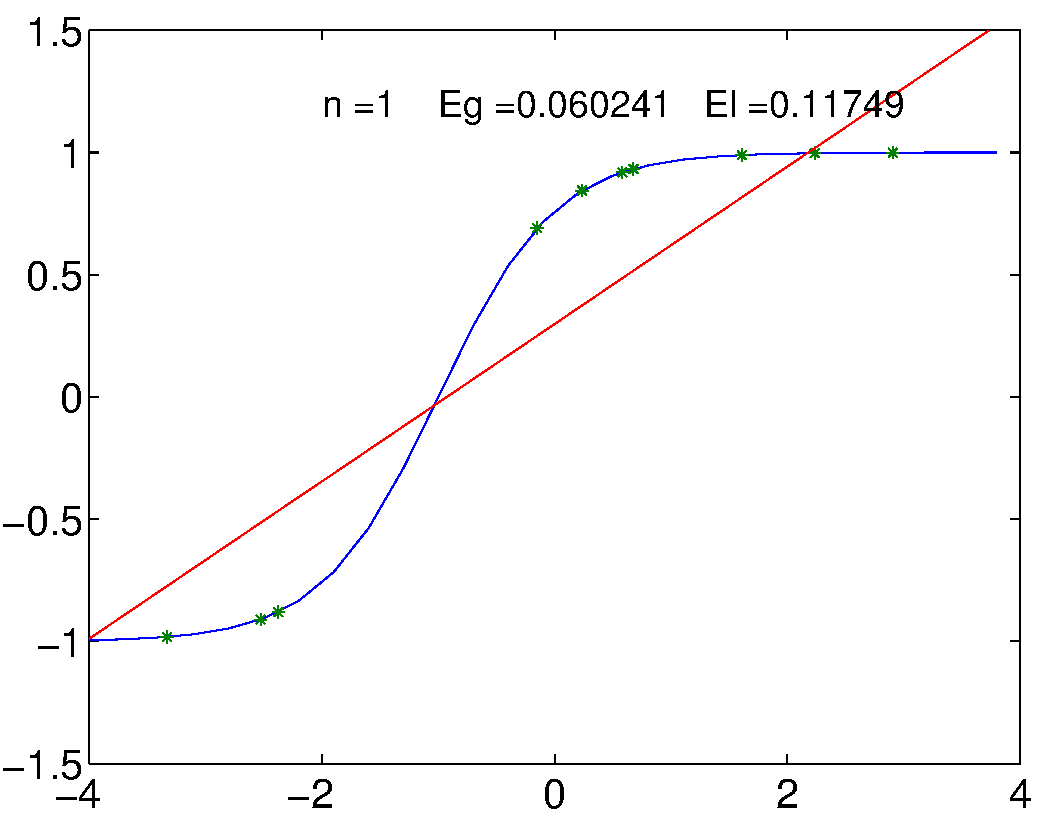
\includegraphics[width=18cm]{bv11}\pause
  \llap{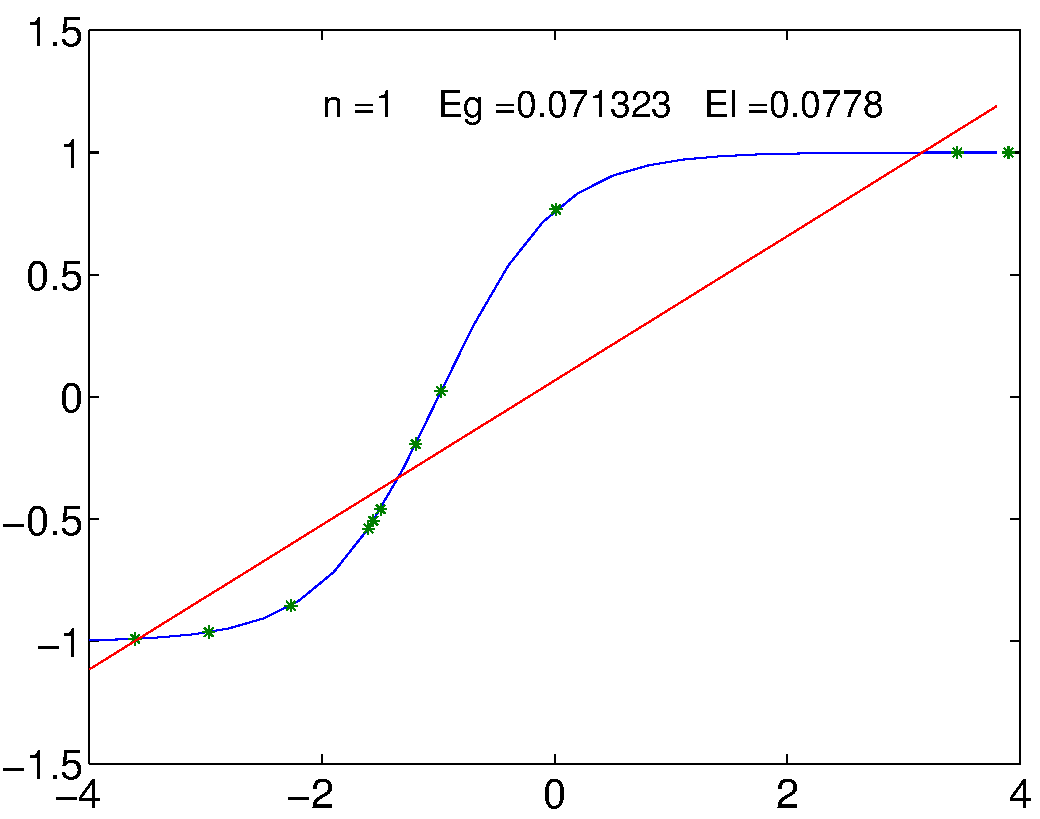
\includegraphics[width=18cm]{bv12}}\pause
  \llap{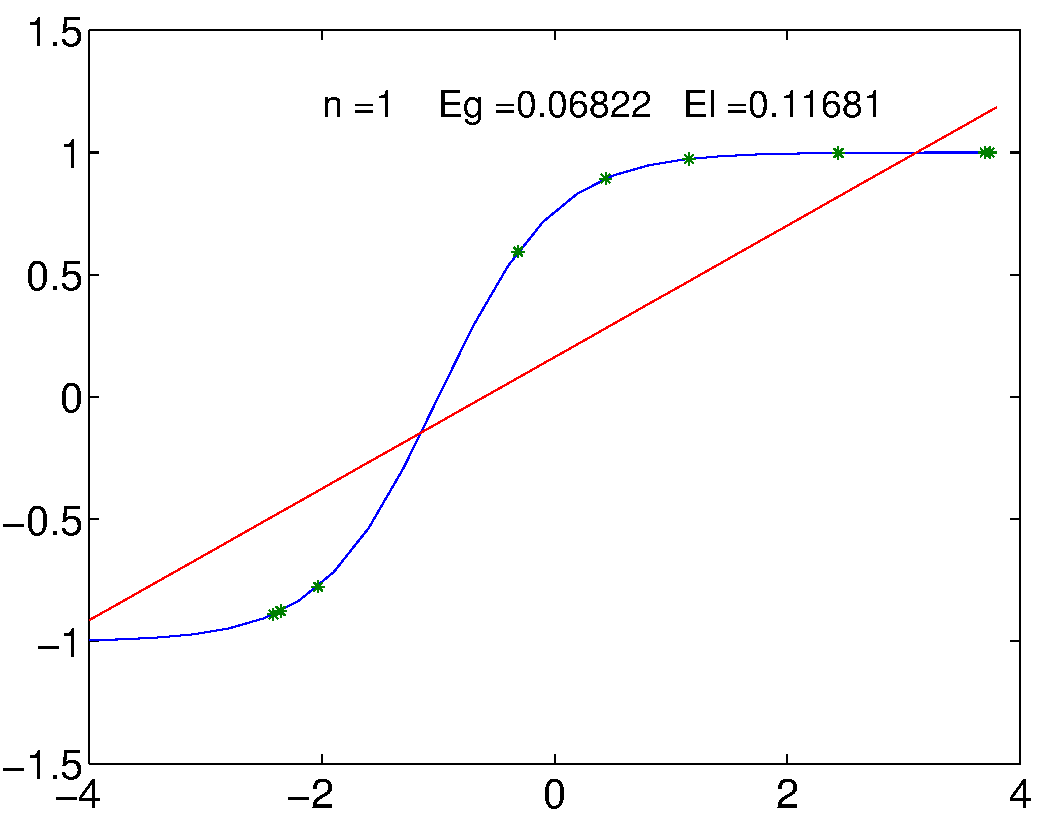
\includegraphics[width=18cm]{bv13}}\pause
  \llap{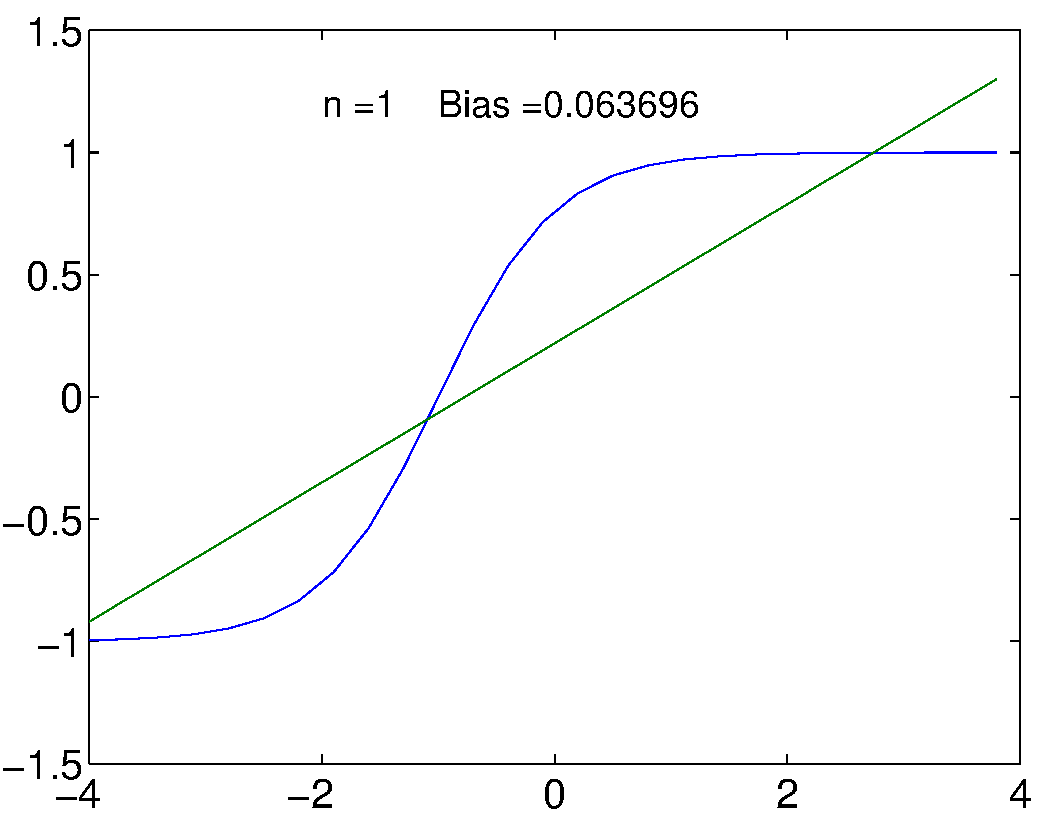
\includegraphics[width=18cm]{bv14}}\pause
\end{center}

\end{slide}



%%%%%%%%%%%%%%%%%%%%%%% Next Slide %%%%%%%%%%%%%%%%%%%%%%%
\whitepage
\begin{slide}
\section[-1]{Regression Example $n=5$}

\pb\pause\pauselevel{=1}
\begin{center}
  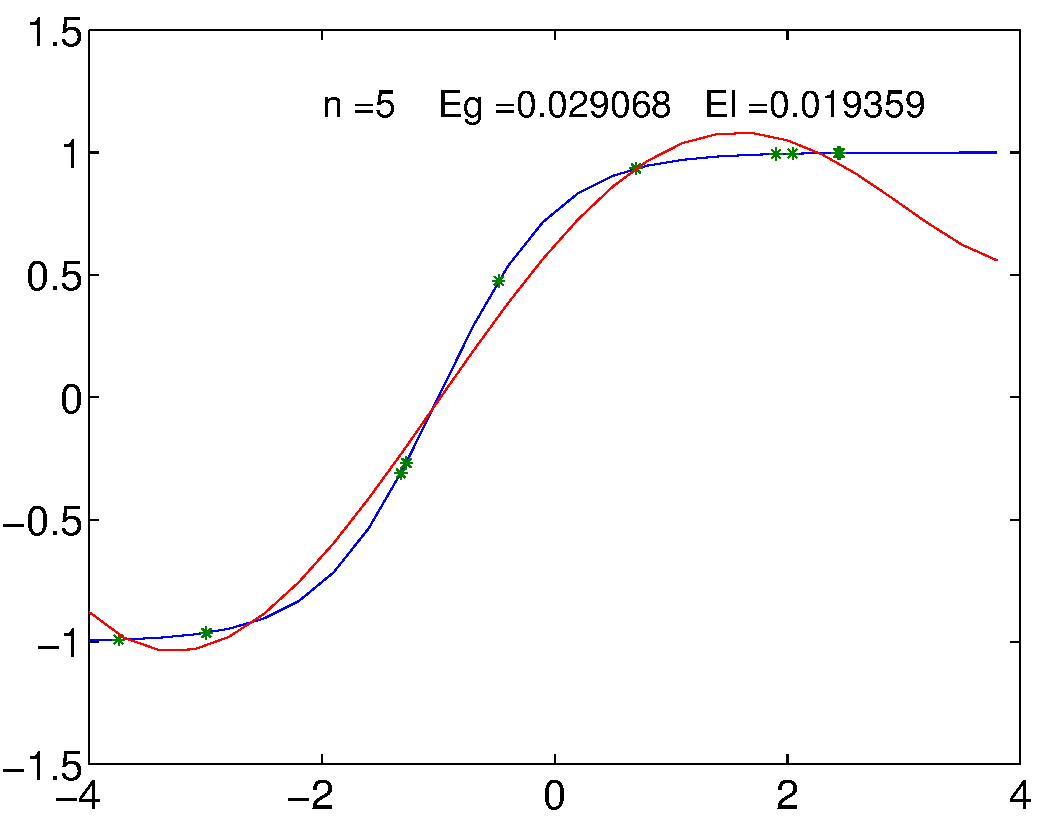
\includegraphics[width=18cm]{bv21}\pause
  \llap{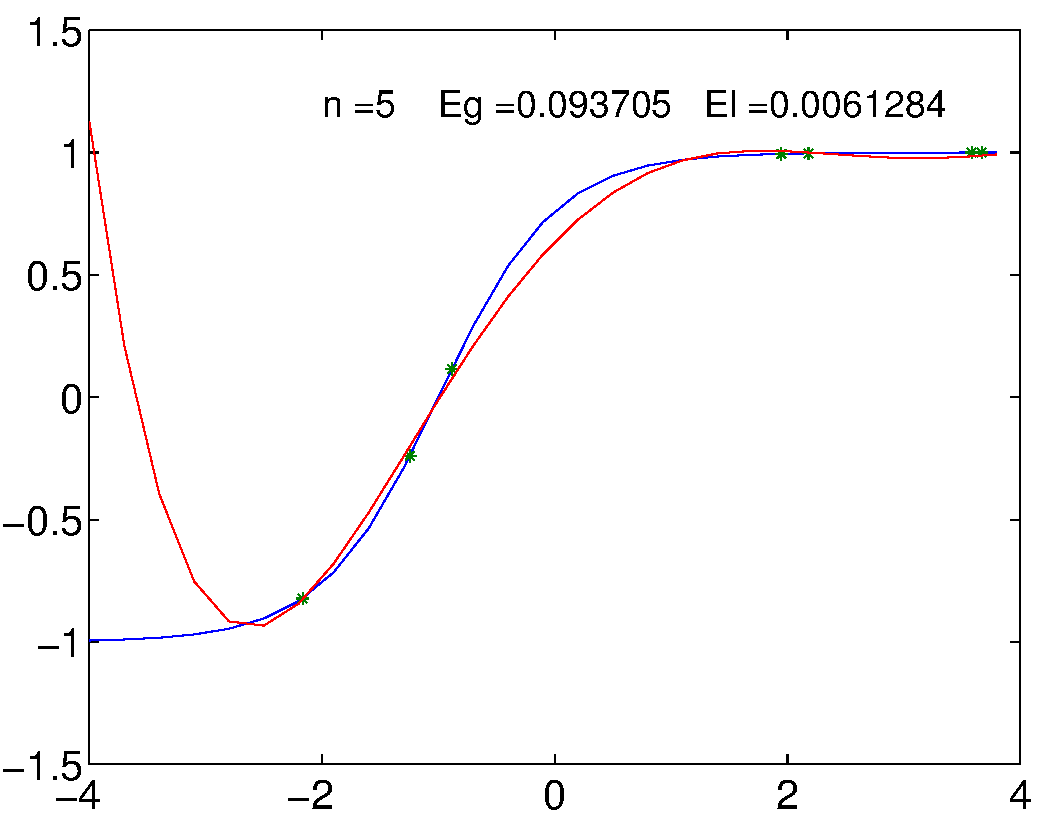
\includegraphics[width=18cm]{bv22}}\pause
  \llap{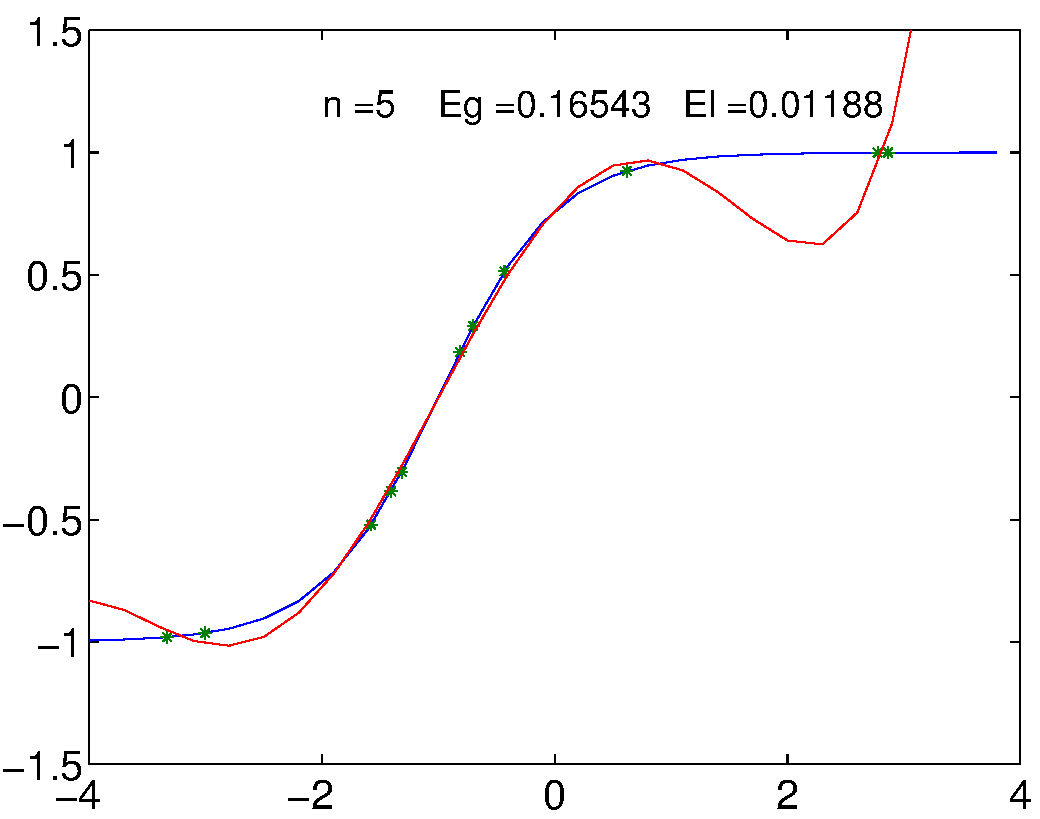
\includegraphics[width=18cm]{bv23}}\pause
  \llap{\toplink{regresscont}{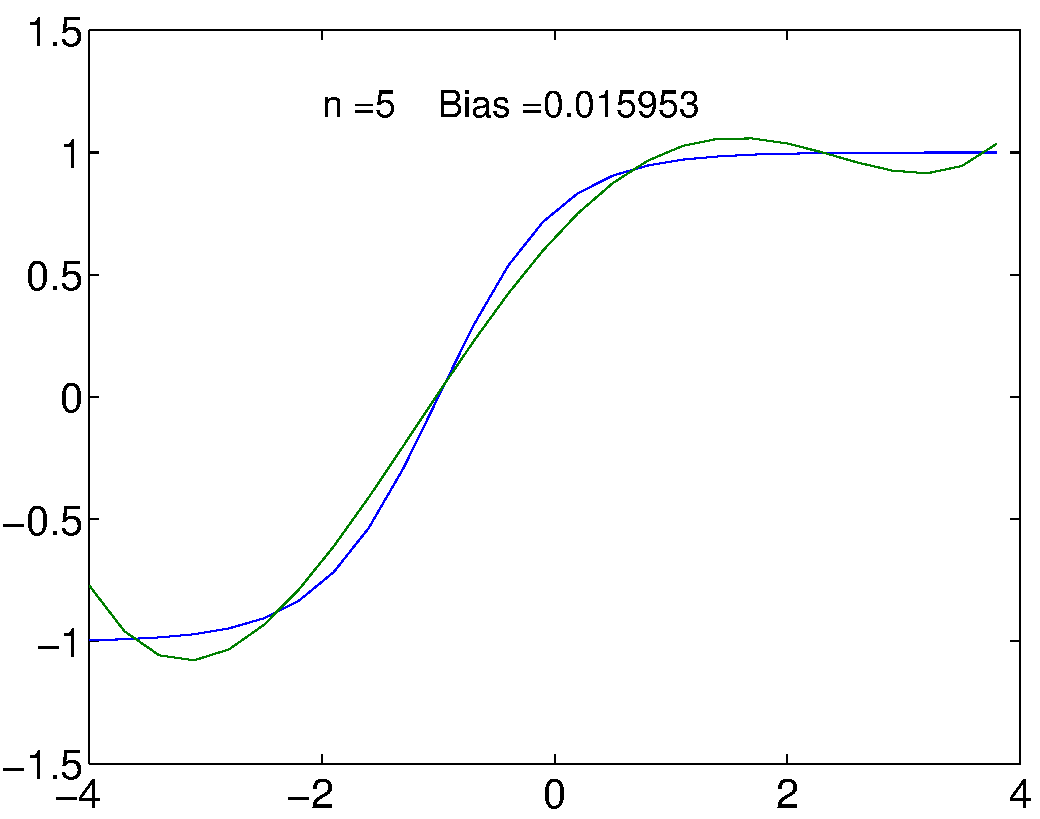
\includegraphics[width=18cm]{bv24}}}\pause
\end{center}
\end{slide}

%%%%%%%%%%%%%%%%%%%%%%% Next Slide %%%%%%%%%%%%%%%%%%%%%%%
\renewcommand{\mypl}[1]{\pauselevel{=#1 :}\pause}
\begin{slide}
\section[-2]{Bias and Variance}

\pb
Consider the expected generalisation for data sets of size $|\mathcal{D}|=m$
\begin{align*}
  \bar{L}_G &= \av[\mathcal{D}]{ L_G(\bm{\theta}_{\mathcal{D}}) } \pause
            = \av[\mathcal{D}]{  \sum_{(\bm{x},y)} \mu(\bm{x},y)\,
              \left(\hat{f}(\bm{x}\vert \bm{\theta}_{\mathcal{D}}) -
              y \right)^2}\pause
  \\
  &=  \sum_{(\bm{x},y)} \mu(\bm{x},y)\,
  \av[\mathcal{D}]{ 
  \left(\hat{f}(\bm{x}\vert \bm{\theta}_{\mathcal{D}}) - y \right)^2}\pause
  \\
      &= \sum_{(\bm{x},y)} \mu(\bm{x},y)\, \av[\mathcal{D}]{
        \left(\mypl{4}\left(\mypl{5}\hat{f}(\bm{x}\vert
        \bm{\theta}_{\mathcal{D}})
        -\hat{f}_m(\bm{x}) \mypl{4}\right)\mypl{5} + \mypl{4}\left(\mypl{5}
        \hat{f}_m(\bm{x}) - y \mypl{4}\right)\mypl{5} \right)^2
        }\mypl{4} \\
            &=  \sum_{(\bm{x},y)} \mu(\bm{x},y) \Biggl(
              \av[\mathcal{D}]{ 
              \left(\hat{f}(\bm{x}\vert \bm{\theta}_{\mathcal{D}}) -
              \hat{f}_m(\bm{x}) \right)^2 + \left(
              \hat{f}_m(\bm{x}) - y \right)^2 }  \\
            & \hspace{5cm} + 2 \, \av[\mathcal{D}]{
              \left(\hat{f}(\bm{x}\vert \bm{\theta}_{\mathcal{D}}) -
              \hat{f}_m(\bm{x}) \right)\left(
              \hat{f}_m(\bm{x}) - y \right) } \Biggr)\mypl{6}
\end{align*}

\end{slide}
%%%%%%%%%%%%%%%%%%%%%%% Next Slide %%%%%%%%%%%%%%%%%%%%%%%

\begin{slide}
\section{Cross Term}

\begin{PauseHighLight}
  \begin{itemize}
  \item The cross term vanishes
  \begin{align*}
  C &= \av[\mathcal{D}]{ \left(\hat{f}(\bm{x}\vert \bm{\theta}_{\mathcal{D}}) -
              \hat{f}_m(\bm{x}) \right) \left(\hat{f}_m(\bm{x}) - y \right) }\pause\\
     &= \av[\mathcal{D}]{ \left(\hat{f}(\bm{x}\vert \bm{\theta}_{\mathcal{D}}) -
              \hat{f}_m(\bm{x}) \right) } \left( \hat{f}_m(\bm{x}) - y \right) \pauseb\\
    &= \left(\av[\mathcal{D}]{\hat{f}(\bm{x}\vert \bm{\theta}_{\mathcal{D}})} -
              \hat{f}_m(\bm{x}) \right) \left(\hat{f}_m(\bm{x}) - y \right)\pauseb\\
     &= \left(\hat{f}_m(\bm{x}) -
              \hat{f}_m(\bm{x}) \right)\left(
              \hat{f}_m(\bm{x}) - y \right)\pauseb
              = 0\pauseb
  \end{align*}
  \item Thus
  \begin{align*}
   \bar{L}_G &= \sum_{(\bm{x},y)} \mu(\bm{x},y)
              \av[\mathcal{D}]{ 
              \left(\hat{f}(\bm{x}\vert \bm{\theta}_{\mathcal{D}}) -
              \hat{f}_m(\bm{x}) \right)^2 + \left(
              \hat{f}_m(\bm{x}) - y \right)^2 }\pauseb
  \end{align*}
  \end{itemize}
\end{PauseHighLight}

\end{slide}



%%%%%%%%%%%%%%%%%%%%%%% Next Slide %%%%%%%%%%%%%%%%%%%%%%%

\begin{slide}
\section[-2]{Bias and Variance}

\begin{PauseHighLight}
  \begin{itemize}
  \item We can write the expected generalisation loss as
    \begin{align*}
      \av[\mathcal{D}]{ L_G(\bm{\theta}_{\mathcal{D}}) }
      &= \sum_{(\bm{x},y)} \mu(\bm{x},y)\, 
      \av[\mathcal{D}]{ \left(\hat{f}(\bm{x}\vert \bm{\theta}_{\mathcal{D}}) -
      \hat{f}_m(\bm{x})\right)^2 } \\
        & \quad \quad +
          \sum_{(\bm{x},y)} \mu(\bm{x},y) \left( \hat{f}_m(\bm{x})
      - y \right)^2 \pause
        = V + B\pause
    \end{align*}
  \item Where $B$ is the bias and $V$ is the variance defined by
    \begin{align*}
      V = \sum_{(\bm{x},y)} \mu(\bm{x},y)\,
      \av[\mathcal{D}]{ \left(\hat{f}(\bm{x}\vert \bm{\theta}_{\mathcal{D}}) -
      \hat{f}_m(\bm{x})\right)^2 }\pause 
    \end{align*}
  \end{itemize}
\end{PauseHighLight}

\end{slide}

%%%%%%%%%%%%%%%%%%%%%%% Next Slide %%%%%%%%%%%%%%%%%%%%%%%

\begin{slide}
\section[-1]{Where Is the Noise?}

\begin{PauseHighLight}
  \begin{itemize}
  \item Suppose $y = f^*(\bm{x}) + \epsilon$ where the noise $\epsilon$ has
    mean 0 and variance $\sigma^2$\pause
  \item Then (the cross term vanishes again, as $\av{\epsilon}=0$)
    \begin{align*}
      B = \sum_{(\bm{x},y)} \mu(\bm{x},y)\bigl(\hat{f}_m(\bm{x}) - y\bigr)^2
      = \sigma^2 + \sum_{\bm{x}} \mu(\bm{x})\bigl(\hat{f}_m(\bm{x}) -
      f^*(\bm{x})\bigr)^2\pause
    \end{align*}
  \item So $\bar{L}_G = \text{noise} + \text{bias}^2 + \text{variance}$,
    the form you may have seen elsewhere\pause
  \item The noise is the same for every machine: we can do nothing
    about it\pause
  \item Here we keep it inside $B$: $\bar{L}_G = B + V$\pause
  \end{itemize}
\end{PauseHighLight}

\end{slide}

%%%%%%%%%%%%%%%%%%%%%%% Next Slide %%%%%%%%%%%%%%%%%%%%%%%

\begin{slide}
\section{Bias-Variance Dilemma}

\begin{PauseHighLight}
  \begin{itemize}
  \item The bias measures the generalisation performance of the
    \textit{mean machine} and is large if the machine is too simple to
    capture the changes in the function we want to learn\pause
  \item The variance measures the variation in the prediction of the
    machines as we change the data set we train on
    \begin{align*}
      V =  \sum_{(\bm{x},y)} \mu(\bm{x},y)\,
      \av[\mathcal{D}]{ \left(\hat{f}(\bm{x}\vert \bm{\theta}_{\mathcal{D}})
      - \hat{f}_m(\bm{x})\right)^2 }\pause
    \end{align*}
  \item \toplink{regress}{The variance is usually large if we have a complex machine}\pause
    \toptarget{regresscont}
  \item Striking the right balance is often the key to getting good
    results\pause 
  \end{itemize}
\end{PauseHighLight}

\end{slide}

%%%%%%%%%%%%%%%%%%%%%%% Next Slide %%%%%%%%%%%%%%%%%%%%%%%

\begin{slide}
\section[-1]{Balancing Bias and Variance}

\begin{PauseHighLight}
  \begin{itemize}
  \item We want to choose a learning machine that is complex enough to
    capture the underlying function we are trying to learn, but
    otherwise as simple as possible\pause
  \item There are a number of tricks to achieve this balance\pause
  \item Some require us to preprocess the data to reduce the number of
    inputs\pause
  \item Some machines cleverly adjust their own complexity\pause
  \item The rest of this lecture: two exact examples, and averaging\pause
  \end{itemize}
\end{PauseHighLight}

\end{slide}

%%%%%%%%%%%%%%%%%%%%%%% Next Slide %%%%%%%%%%%%%%%%%%%%%%%
\Outline % Shrinkage and Ridge Regression
%%%%%%%%%%%%%%%%%%%%%%% Next Slide %%%%%%%%%%%%%%%%%%%%%%%

\begin{slide}
\section[-1]{Shrinking an Estimate}

\begin{PauseHighLight}
  \begin{itemize}
  \item The simplest learning problem: estimate the mean $\theta$ of a
    distribution with variance $\sigma^2$ from $m$ samples\pause
  \item The sample mean $\bar{x}$ is unbiased with variance
    $\sigma^2/m$\pause
  \item Try the deliberately biased $\hat{\theta} = c\,\bar{x}$ with
    $0\leq c\leq1$
    \begin{align*}
      \av{\bigl(\hat{\theta}-\theta\bigr)^2} =
      \underbrace{(1-c)^2\,\theta^2}_{\text{bias}^2} +
      \underbrace{c^2\,\frac{\sigma^2}{m}}_{\text{variance}}\pause
    \end{align*}
  \item At $c=1$ the derivative is $2\sigma^2/m>0$: shrinking a
    little \emph{always} reduces the error\pause
  \item The best $c$ depends on the unknown $\theta$, so in practice we
    choose it by validation\pause
  \end{itemize}
\end{PauseHighLight}

\end{slide}

%%%%%%%%%%%%%%%%%%%%%%% Next Slide %%%%%%%%%%%%%%%%%%%%%%%

\begin{slide}
\section[-1]{Ridge Regression}

\begin{PauseHighLight}
  \begin{itemize}
  \item Data $\bm{y} = \mat{X}\bm{w}^* + \bm{\epsilon}$, with noise of
    variance $\sigma^2$ on each target\pause
  \item Ridge regression minimises $\|\mat{X}\bm{w} - \bm{y}\|^2 +
    \eta\,\|\bm{w}\|^2$, giving
    \begin{align*}
      \hat{\bm{w}} = \bigl(\mat{X}^\tr\mat{X} + \eta\,\mat{I}\bigr)^{-1}
      \mat{X}^\tr\bm{y}\pause
    \end{align*}
  \item $\eta = 0$ is least squares: unbiased, but how variable?\pause
  \item Use the SVD $\mat{X} = \mat{U}\mat{S}\mat{V}^\tr$ and work in
    the basis of the columns of $\mat{V}$, where everything
    separates\pause
  \end{itemize}
\end{PauseHighLight}

\end{slide}

%%%%%%%%%%%%%%%%%%%%%%% Next Slide %%%%%%%%%%%%%%%%%%%%%%%

\begin{slide}
\section[-2]{Ridge Through the SVD}

\begin{PauseHighLight}
  \begin{itemize}\squeeze
  \item Write $w_k^* = \bm{v}_k^\tr\bm{w}^*$ for the component of
    $\bm{w}^*$ along $\bm{v}_k$; since $\bm{u}_k^\tr\bm{y} = s_k w_k^* +
    \bm{u}_k^\tr\bm{\epsilon}$, the same component of the estimate is
    \begin{align*}
      \hat{w}_k = \frac{s_k\,\bm{u}_k^\tr\bm{y}}{s_k^2+\eta}, \qquad
      \av{\hat{w}_k} = \frac{s_k^2}{s_k^2+\eta}\,w_k^*, \qquad
      \mathrm{Var}(\hat{w}_k) = \frac{\sigma^2 s_k^2}{(s_k^2+\eta)^2}\pause
    \end{align*}
  \item So the expected squared error of the weights is
    \begin{align*}
      \av{\|\hat{\bm{w}} - \bm{w}^*\|^2} = \sum_k
      \underbrace{\Bigl(\frac{\eta}{s_k^2+\eta}\Bigr)^2 {w_k^*}^2}_{\text{bias}^2}
      + \underbrace{\frac{\sigma^2 s_k^2}{(s_k^2+\eta)^2}}_{\text{variance}}\pause
    \end{align*}
  \item With $\eta=0$ the variance is $\sum_k\sigma^2/s_k^2$: small
    singular values (ill-conditioning) make it huge\pause{}; $\eta$
    shrinks exactly those directions, trading a little bias for a large
    drop in variance\pauseb
  \end{itemize}
\end{PauseHighLight}

\end{slide}

%%%%%%%%%%%%%%%%%%%%%%% Next Slide %%%%%%%%%%%%%%%%%%%%%%%

\begin{slide}
\section[-2]{Choosing $\eta$}

\begin{center}
  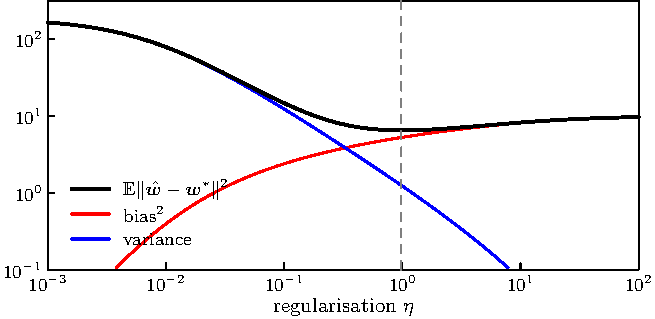
\includegraphics[width=0.85\linewidth]{ridgeBV-0}
\end{center}
\begin{PauseHighLight}
  \begin{itemize}\squeeze
  \item Ten singular values from 3 down to 0.1, $\sigma=1$: least
    squares has error 188, the best $\eta\approx1$ gives 6.5\pause
  \item In practice choose $\eta$ by cross-validation\pause
  \end{itemize}
\end{PauseHighLight}

\end{slide}

%%%%%%%%%%%%%%%%%%%%%%% Next Slide %%%%%%%%%%%%%%%%%%%%%%%
\Outline % Ensembles
%%%%%%%%%%%%%%%%%%%%%%% Next Slide %%%%%%%%%%%%%%%%%%%%%%%

\begin{slide}
\section[-1]{Averaging Reduces Variance}

\begin{PauseHighLight}
  \begin{itemize}
  \item An \emph{ensemble} averages $M$ predictors,
    $\bar{f}_M(\bm{x}) = \frac{1}{M}\sum_{i=1}^M f_i(\bm{x})$, trained
    with different randomness\pause
  \item Averaging does not change the mean, so the bias is
    unchanged\pause
  \item If each $f_i(\bm{x})$ has variance $s^2$ and each pair has
    correlation $\rho$
    \begin{align*}
      \mathrm{Var}\bigl(\bar{f}_M(\bm{x})\bigr) = \rho\,s^2 +
      \frac{1-\rho}{M}\,s^2\pause
    \end{align*}
  \item More members remove the second term, but correlation sets a
    floor $\rho\,s^2$\pause
  \item So we want members that are good \emph{and} different\pause
  \end{itemize}
\end{PauseHighLight}

\end{slide}

%%%%%%%%%%%%%%%%%%%%%%% Next Slide %%%%%%%%%%%%%%%%%%%%%%%

\begin{slide}
\section[-1]{Bagging, Forests and Deep Ensembles}

\begin{PauseHighLight}
  \begin{itemize}
  \item \emph{Bagging}: train each member on a bootstrap resample of the
    data (sampled with replacement)\pause
  \item \emph{Random forests}: bagged decision trees that also choose
    each split from a random subset of the features\pause{}---each tree
    is worse, but the trees are less correlated\pauseb
  \item \emph{Deep ensembles}: train several networks on the same data
    from different random initialisations\pause
  \item The spread of the members' predictions is a useful measure of
    uncertainty\pause
  \item Ensembles of high-variance, low-bias machines are among the
    most reliable methods in practice\pause
  \end{itemize}
\end{PauseHighLight}

\end{slide}

%%%%%%%%%%%%%%%%%%%%%%% Next Slide %%%%%%%%%%%%%%%%%%%%%%%

\begin{slide}
\section[-2]{Lessons}

\begin{PauseHighLight}
  \begin{itemize}
  \item The expected generalisation loss splits into bias plus
    variance\pause
  \item One of the most useful intuitions about what works is the
    bias-variance framework\pause
  \item A biased estimate can beat an unbiased one: shrinkage, ridge
    regression\pause
  \item The bias is high for simple machines that can't capture the
    data\pause
  \item The variance is high for complex machines that are sensitive
    to the training set\pause
  \item Averaging (ensembles) reduces variance without adding
    bias\pause
  \end{itemize}
\end{PauseHighLight}

\end{slide}


%%% Local Variables:
%%% TeX-master: "lectures"
%%% End:

\end{document}
